\chapter{Dise\~no de experimentos de microarrays}

En este cap\'itulo se examinan un componentes clave del an\'alisis de microarrays el dise\~no de experimentos que, no tan s\'olo es
crucial para una buena recogida de informaci\'on sino que marca todo el proceso desde el preprocesado al an\'alisis final.

\section{Fuentes de variabilidad}

Los datos gen\'omicos son muy variables.


\textD{Figura \ref{c04variabilitySources}}{Geschwind (\cite{geschwind:2002} ilustra algunas posibles fuentes de variabilidad, desde que se inicia el experimento hasta que se lee la informaci\'on con el sacnner.}

\vspace{-0.5cm}
\begin{figure}[!h]
\titolfigura[0cm]{Figura \ref{c04variabilitySources}. Proceso de an\'alisis de microarrays}
\label{c04variabilitySources}
\fbox{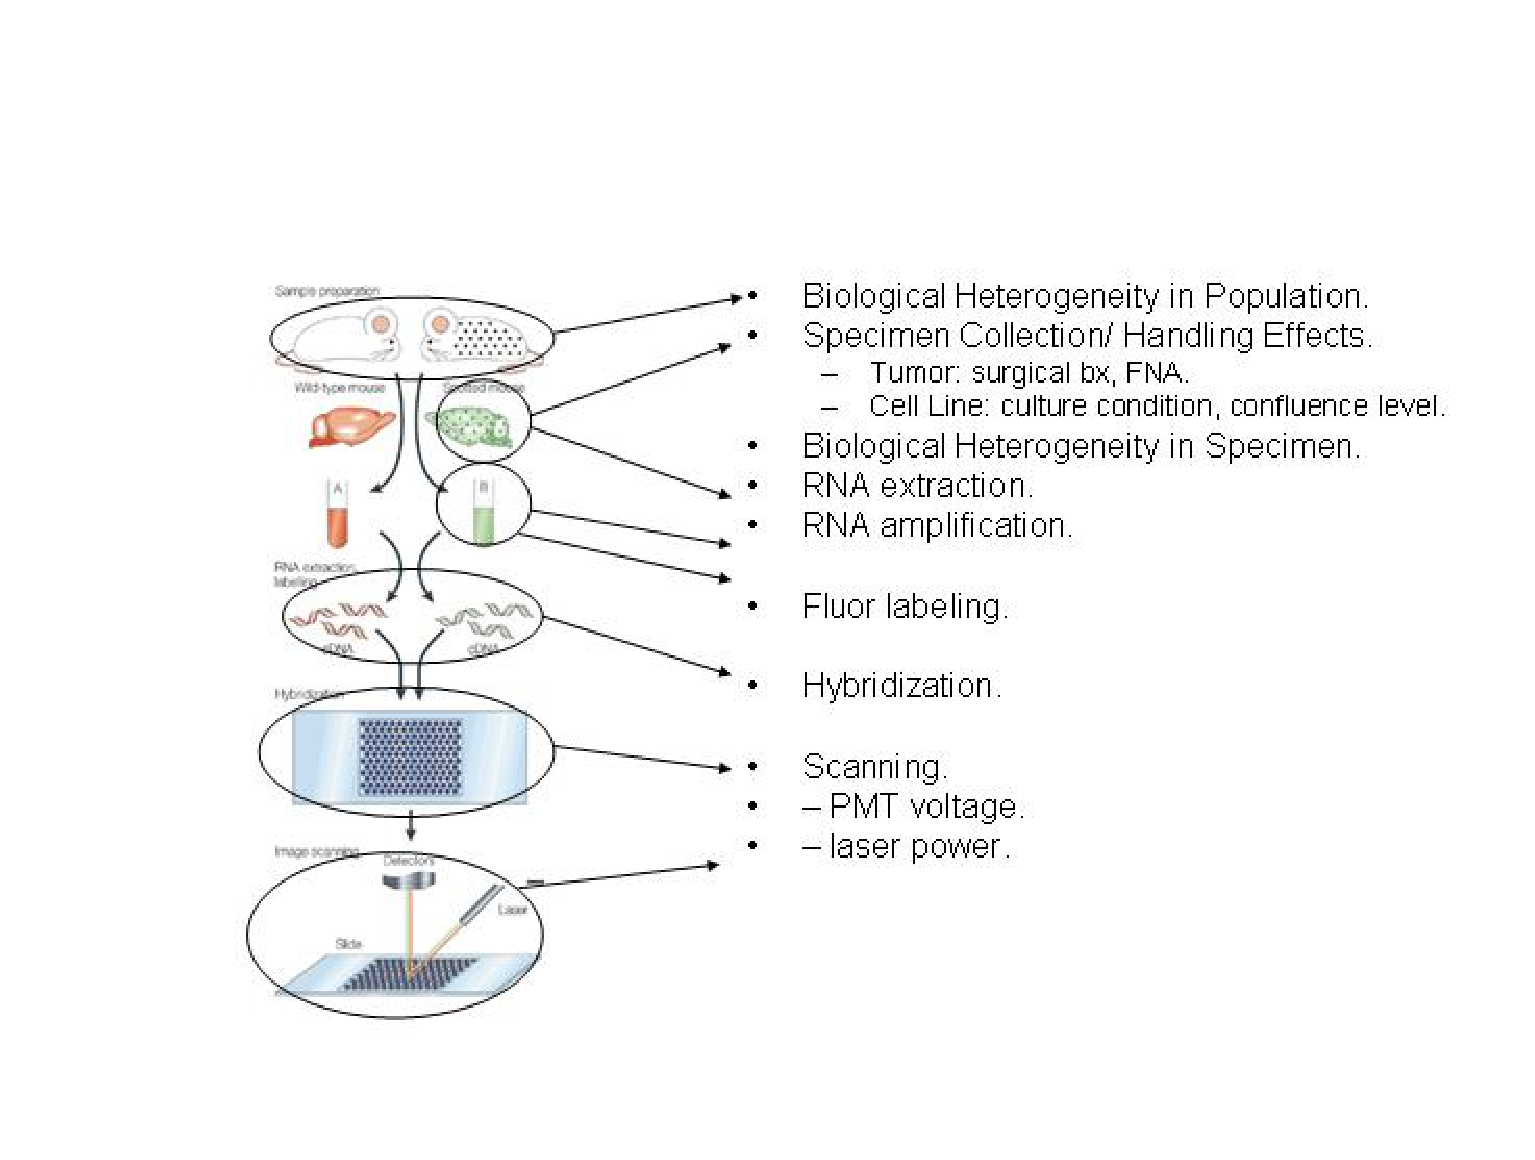
\includegraphics[height=6cm,width=0.75\linewidth]{epsimages/c04variabilitySources.eps}}
\end{figure}


Habitualmente, en la mayor parte de situaciones experimentales, podemos
distinguir entre variabilidad sistem\'atica y aleatoria.

La variabilidad sistem\'atica es principalmente debida a procesos t\'ecnicos
mientras que la variabilidad aleatoria es atribuible tanto a razones t\'ecnicas
como biol\'ogicas. Podemos encontrar ejemplos de variabilidad sistem\'atica en la
extracci\'on del ARN, marcaje o fotodetecci\'on. La variabilidad aleatoria puede
estar relacionada con muchos factores tales como la calidad del ADN o las
caracter\'isticas biol\'ogicas de las muestras.

La manera natural de manejar la variabilidad aleatoria es, por supuesto, la
utilizaci\'on de un dise\~no experimental apropiado y el apoyo para obtener
conclusiones de unas herramientas estad\'isticas adecuadas. Los problemas
relacionados con el dise\~no de los experimentos los discutiremos en esta secci\'on
y los relacionados con la aplicaci\'on de m\'etodos estad\'isticos ser\'an tratados
en la secci\'on  ~\ref{m\'etodos estad\'isticos}.

Tradicionalmente, se estiman las correcciones de la variabilidad sistem\'atica
a partir de los datos, en lo que se llama gen\'ericamente ''calibrado''. En este
contexto, hablaremos de ``normalizaci\'on'', que se tratar\'a en la secci\'on
 ~\ref{preprocesamiento}.

\section{Principales conceptos en Dise\~no de Experimentos}

Vamos a plantear alguna definiciones de conceptos que aparecen de forma usual cuando se plantea un dise\~no:
\begin{itemize}

\item \textbf{Unidad experimental}: Entidad f\'isica a la que se aplica un tratamiento, de forma independiente al resto de unidades. En cada unidad experimental se pueden realizar una medida o varias medidas, en este caso distinguiremos entre unidades experimetales y unidades observacionales. .
\item \textbf{Factor}: son las variables independientes que pueden influir en la variabilidad de la variable de inter\'es.
\item \textbf{Factor tratamiento}: es un factor del que interesa conocer su influencia en la respuesta.
 \item \textbf{Factor bloque}: es un factor en el que no se est\'a interesado en conocer su influencia en la respuesta pero se supone que \'esta existe y se quiere controlar para disminuir la variabilidad residual.
 \item \textbf{Niveles}: cada uno de los resultados de un factor. Seg\'un sean elegidos por el experimentador o elegidos al azar de una amplia poblaci܇n se denominan factores de efectos fijos o factores de efectos  aleatorios.
 \item \textbf{Tratamiento}: es una combinaci\'on espec\'ifica de los niveles de los factores en estudio. Son, por tanto, las condiciones experimentales que se desean comparar en el experimento. En un dise\~no con un \'unico factor son los distintos niveles del factor y en un dise\~no con varios factores son las distintas combinaciones de niveles de los factores.
 \item \textbf{Tama\~no del Experimento}: es el n\'umero total de observaciones recogidas en el dise\~no.
 \end{itemize}

 \section{Principios b\'asicos en el dise\~no del experimento}
 Al planificar un experimento, aparte de la replicaci\'on, hay tres principios b\'asicos que se deben tener siempre en cuenta: 
La replicaci\'on, el control local o ``bloqueo'' y la \textit{aleatorizaci\'on}.
Aplicados correctamente dichos principios garantizan dise\~nos experimentales eficientes.


\section{Replicaci\'on\label{replicacion}}

La replicaci\'on o repetici\'on de un experimento de forma id\'entica en un n\'umero determinado de unidades, es la que
permite la realizaci\'on de un posterior an\'alisis estad\'istico.
La utilizaci\'on de r\'eplicas ss importante para incrementar la precisi\'on, obtener suficiente potencia en los tests y como base para los
procedimientos de inferencia. Normalmente, distinguimos dos tipos de r\'eplicas en el an\'alisis de microarrays:

\begin{itemize}
\item \emph{La replicaci\'on t\'ecnica} se utiliza cuando estamos tratando
r\'eplicas del mismo material biol\'ogico. Puede ser tanto la replicaci\'on
de spots en el mismo chip como la de diferentes alicuotas de la misma muestra
hibridadas en diferentes microarrays.

\item \emph{Replicaci\'on biol\'ogica} se da cuando se toman medidas de m\'ultiples
muestras.

\end{itemize}
La replicaci\'on t\'ecnica permite la estimaci\'on del error a nivel de medida, mientras que
la  replicaci\'on biol\'ogica permite estimar la variabilidad a nivel de poblaci\'on.


\textD{Figura \ref{c04replicas}}{R\'eplicas biol\'ogicas vs t\'ecnicas}

\vspace{-0.5cm}
\begin{figure}[!h]
\titolfigura[0cm]{Figura \ref{c04replicas}.}
\label{c04replicas}
\fbox{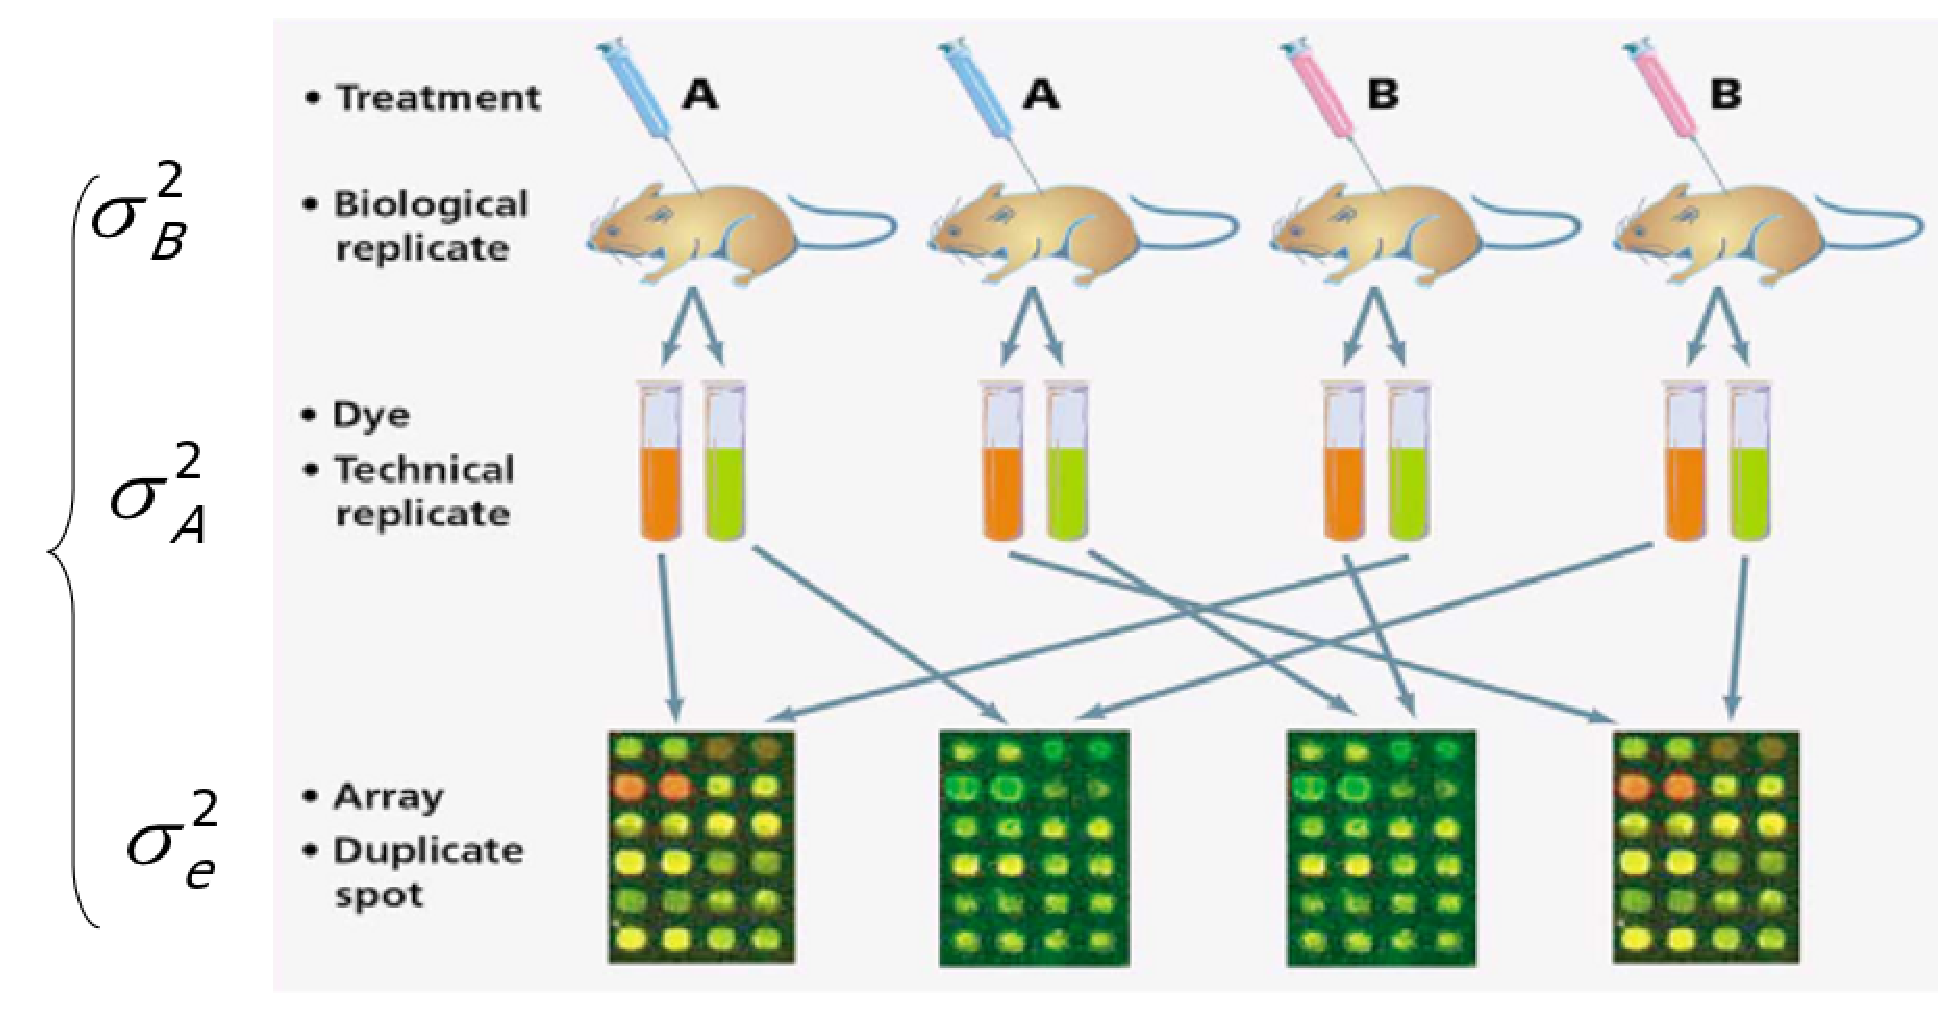
\includegraphics[height=6cm,width=0.75\linewidth]{epsimages/c04replicas.eps}}
\end{figure}


\subsection{Potencia y tama\~no de la muestra\label{samplesize}}

Sorprendentemente, los primeros experimentos de microarrays utilizaban pocas o
ninguna r\'eplica biol\'ogica. La principal explicaci\'on para este hecho - adem\'as
de la falta de conocimiento estad\'istico - fu\'e el alto coste de cada microarray.
En pocos a\~nos, la necesidad de las r\'eplicas ha llegado a ser indiscutible, y al
mismo tiempo, el coste de los chips ha disminuido considerablemente. Actualmente,
es normal la utilizaci\'on de, al menos, tres a cinco r\'eplicas por condici\'on
experimental, aunque a este consenso se ha llegado m\'as por razones emp\'iricas que
por la disponibilidad de modelos apropiados para el an\'alisis de la potencia y
tama\~no de la muestra.

Recientemente, se ha producido una importante afluencia de art\'iculos describiendo
m\'etodos para el an\'alisis de la potencia y tama\~no de la muestra. A pesar de su
variedad, ning\'un m\'etodo aparece como candidato claro para ser utilizado en
situaciones pr\'acticas. Esto se debe, probablemente, a la complejidad de los
datos de microarrays, b\'asicamente por que los genes no son independientes. Por
tanto, estas estructuras de correlaci\'on existen en los datos, pero la mayor parte
de las dependencias son desconocidas por lo que la estimaci\'on de estas estructuras
es muy complicada.

Como indicaba Allison (~\cite{Allison:2006a}) aunque no hay consenso sobre que
procedimiento es mejor para determinar el tama\~no de las muestras, s\'i que lo hay
sobre la conveniencia de realizar el an\'alisis de la potencia, y, por supuesto,
sobre el hecho de que un mayor n\'umero de replicas generalmente proporcionan
una mayor potencia.

\subsection{Pooling\label{pooling}}

En el contexto de los microarrays, llamamos "pooling" a la combinaci\'on de mARN
de diferentes casos en una \'unica muestra. Hay dos razones a favor de ello, una,
es que, a veces, no hay suficiente ARN disponible y esta es la \'unica forma de
conseguir suficiente material para construir los arrays, otra, m\'as controvertida,
es la creencia que la variabilidad entre arrays puede reducirse por "pooling".
La justificaci\'on es que combinar muestras equivale a promediar expresiones, y
como ya se conoce, el promedio es menos variable que los valores individuales. A
pesar de la debilidad de este argumento, es verdad que en ciertas situaciones el
pooling puede ser apropiado y, recientemente, muchos estad\'isticos han dedicado
sus esfuerzos a tratar de responder la pregunta ``to pool or not to pool"
(~\cite{Kerr:2001a}). Por ejemplo, si la variabilidad biol\'ogica est\'a altamente
relacionada con el error en las medidas, y las muestras biol\'ogicas tienen un
coste m\'inimo en comparaci\'on con el de los arrays, una apropiada estrategia de
"pooling" puede ser claramente eficiente en costes.

De todos modos, el "pooling" no se deber\'ia usar en cualquier tipo de estudios.
Si el objetivo es comparar expresiones medias (ver m\'as adelante '' comparaci\'on
de clases''), puede funcionar adecuadamente, pero se deber\'ia claramente evitar
cuando el objetivo del experimento es construir predictores que se basen en
caracter\'isticas individuales.


 \subsubsection{Aleatorizaci\'on}

Se entiende por aleatorizar la asignaci\'on de todos los factores al azar a las unidades experimentales. Co ello se consigue disminuir el efecto de los factores no controlados por el experimentador en el dise\~no experimental y que podr\'ian  influir en los resultados.

Las ventajas de aleatorizar los factores no controlados son:
\begin{itemize}
  \item Transforma la variabilidad sistem\'atica no planificada en variabilidad no planificada o ruido aleatorio. Dicho de otra forma, aleatorizar previene contra la introducci\'on de sesgos en el experimento.
  \item Evita la dependencia entre observaciones al aleatorizar los instantes de recogida muestral.
  \item Valida muchos de los procedimientos estad\'isticos m\'as comunes.
\end{itemize}

\subsubsection{Bloquear}

Hace referencia a dividir o particionar las unidades experimentales en grupos llamados bloques de modo que las observaciones realizadas en cada bloque se realicen bajo condiciones experimentales lo m\'as parecidas posibles.
A diferencia de lo que ocurre con los factores tratamiento, el experimentador no est\'a interesado en investigar las posibles diferencias de la respuesta entre los niveles de los factores bloque.

Bloquear es una buena estrategia siempre y cuando sea posible dividir las unidades experimentales en grupos de unidades similares. La ventaja de bloquear un factor que se supone que tiene una clara influencia en la respuesta pero en el que no se est\'a interesado, es que convierte la variabilidad sistem\'atica no planificada en variabilidad sistem\'atica planificada.


\section{Dise\~nos experimentales para microarrays de dos colores}

En arrays de dos colores, se aplican dos condiciones experimentales a cada array.
Esto permite la estimaci\'on del efecto del array, como el efecto de bloqueo.
En Affymetrix u otro array de un canal, cada condici\'on se aplica a un
chip separado, imposibilitando la estimaci\'on del efecto de los microarrays, lo
cual, por otra parte, se considera que tiene una relaci\'on muy peque\~na en el
tratamiento de los efectos debido al proceso industrial utilizado para fabricar
estos chips.

Como consecuencia de lo anterior, los experimentos que usan arrays de un canal
se consideran ``estandar'', por lo que se les pueden aplicar los conceptos y t\'ecnicas tradicionales de
dise\~no de experimentos .


Los arrays de dos canales presentan una situaci\'on m\'as complicada. Por una parte los
``dos colores'' no son sim\'etricos, es decir, con la misma cantidad de material,
un array hibridado con uno u otro color, sea Cy5 o Cy3, emitir\'a se\~nales con
diferente intensidad. La forma normal de manejar este problema es
 \emph{dye--swapping} que consiste en utilizar para una misma comparaci\'on dos
arrays con dyes cambiados, es decir, si en el primer array la muestra 1 se marca
con Cy3 y la muestra 2 con Cy5, con las muestras del segundo array se hace al
rev\'es (ver figura \ref{c04dyelabels}).


\textD{Figura \ref{c04dyelabels}}{(a) Representaci\'on simplificada de un dise\~no. Cada flecha representa
  un array de dos canales en el que el origen indica el marcaje con Cy3.
  (b) Dye swapping.}

\vspace{-0.5cm}
\begin{figure}[!h]
\titolfigura[0cm]{Figura \ref{c04dyelabels}.}
\label{c04dyelabels}
\fbox{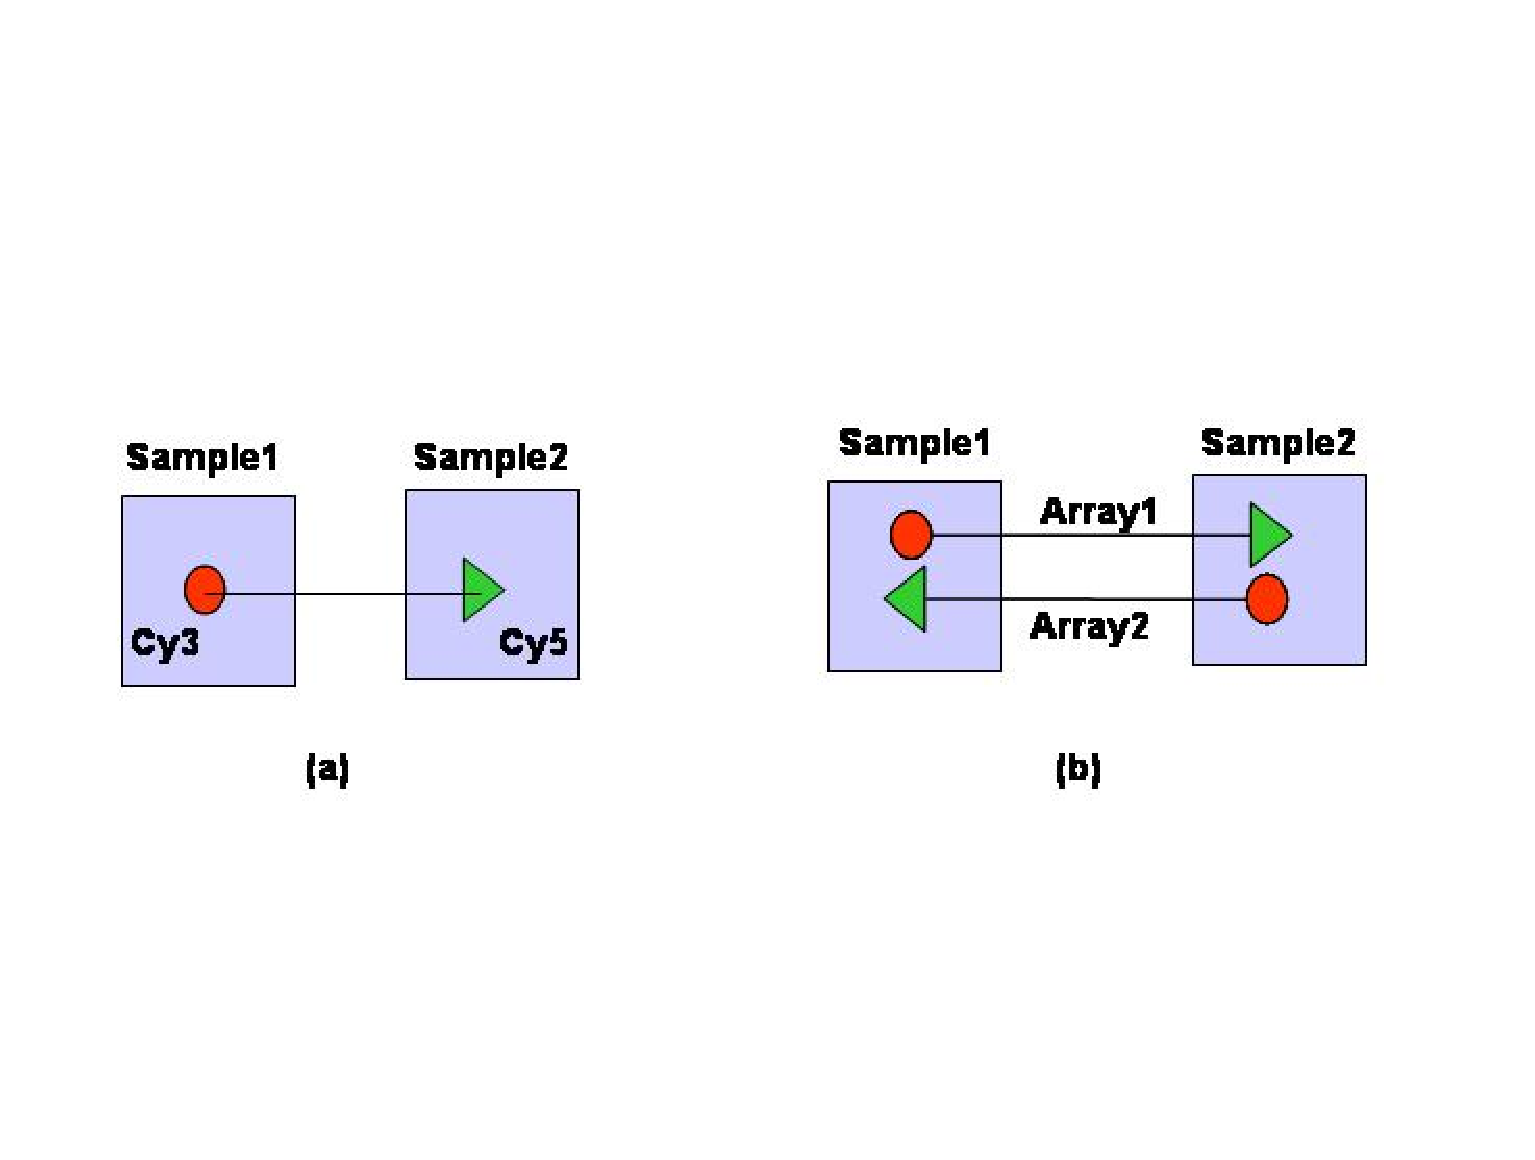
\includegraphics[height=6cm,width=0.75\linewidth]{epsimages/c04dyelabels.eps}}
\end{figure}


Por otra parte, el hecho de que solo se puedan aplicar dos condiciones a cada
array complica el dise\~no, ya sea porque normalmente hay m\'as de dos condiciones,
o porque no es recomendable hibridar directamente dos muestras en un array,
creando pares artificiales.

El problema de la asignaci\'on eficiente de muestras a microarrays, dado un n\'umero
de condiciones a comparar y un n\'umero fijo de arrays disponibles, ha sido
estudiado de forma exhaustiva.

El dise\~no utilizado m\'as comunmente en la comunidad biol\'ogica es el
 \emph{dise\~no de referencia} en el que cada condici\'on de inter\'es se compara
 con muestras tomadas de alguna referencia estandar com\'un a todos las arrays.
(ver figura \ref{c04referencevsloop} (a)).


\textD{Figura \ref{c04referencevsloop}}{(a) Dise\~no de referencia.  (b) Dise\~no en loop.}

\vspace{-0.5cm}
\begin{figure}[!h]
\titolfigura[0cm]{Figura \ref{c04referencevsloop}. Dise\~no de arrays.}
\label{c04referencevsloop}
\fbox{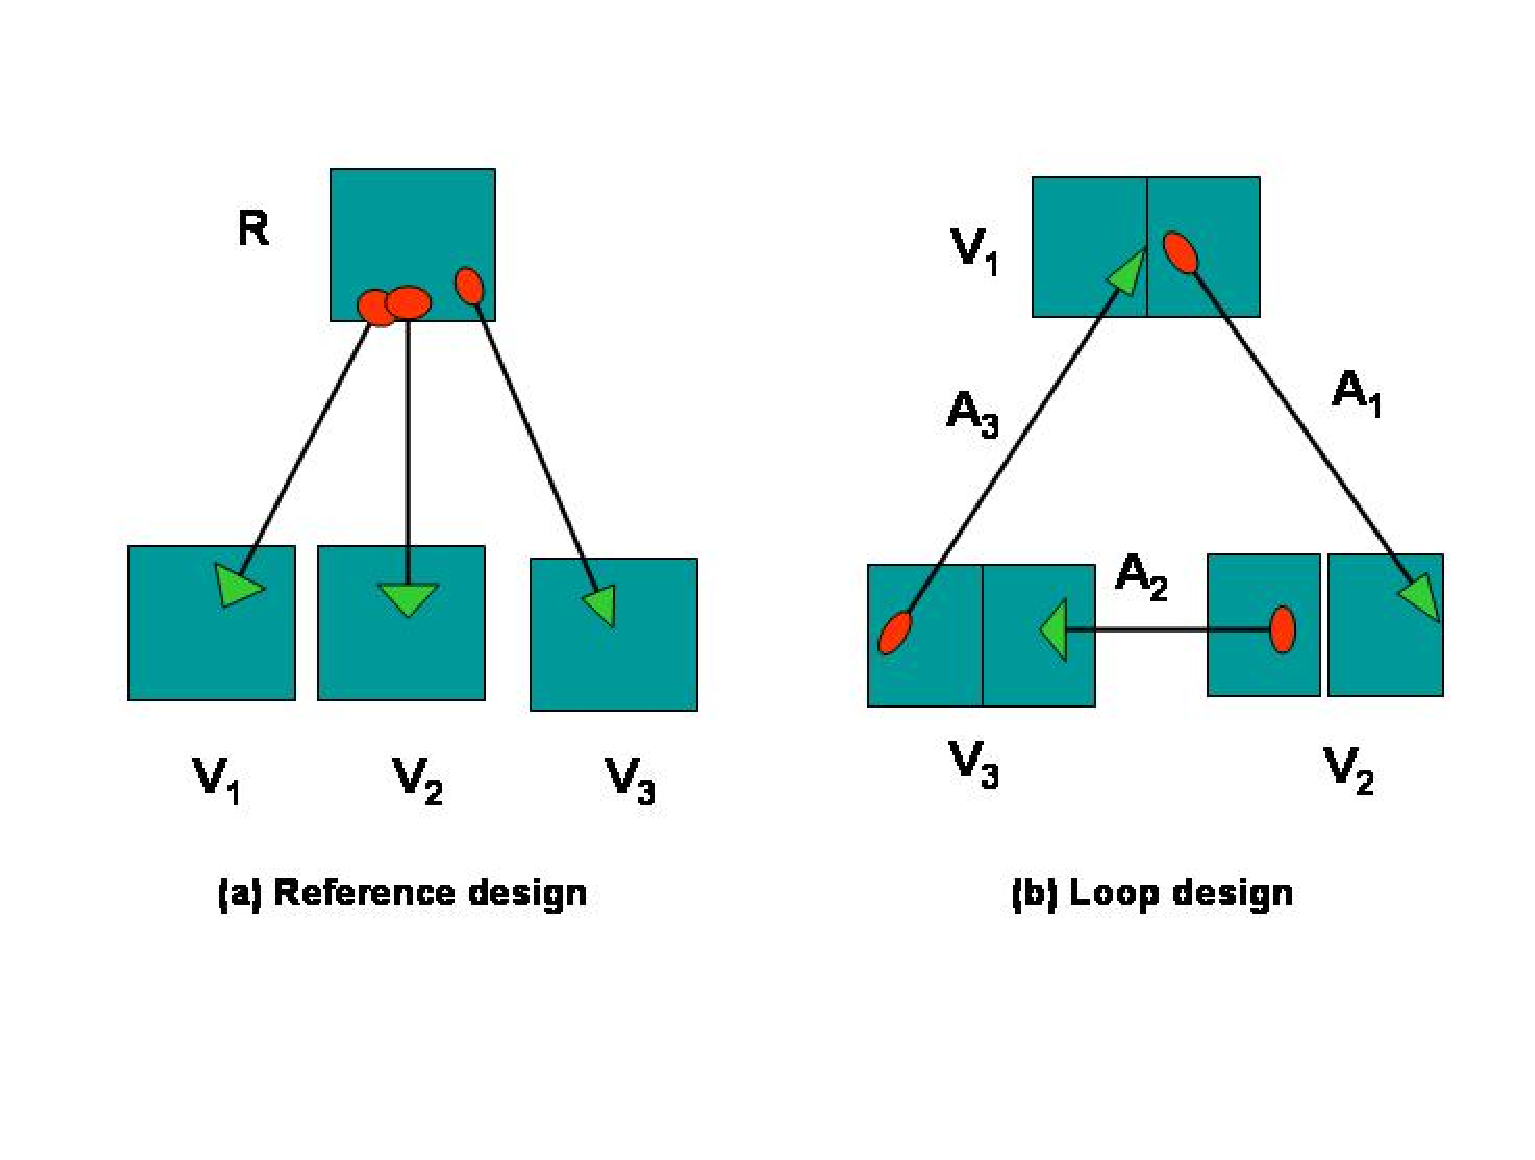
\includegraphics[height=6cm,width=0.75\textwidth]{epsimages/c04referencevsloop.eps}}
\end{figure}

Los dise\~nos de referencia permiten hacer comparaciones indirectas entre
condiciones de inter\'es. La critica m\'as importante a esta aproximaci\'on es que el
50\% de las fuentes de hibridaci\'on se utilizan para  producir la se\~nal del grupo
control, de un inter\'es no intr\'inseco para los bi\'ologos.
En contraste, un dise\~no en loop compara dos condiciones a trav\'es de otra cadena
de condiciones, por lo que elimina la necesidad de una muestra de referencia
 (ver figura \ref{c04referencevsloop}(b)).



